\documentclass{article}
\usepackage[utf8]{inputenc}
\usepackage{fullpage}
\usepackage{graphicx}
\title{Operating System-2 \\  Assignment 1}
\author{Parallel Sorting using Multi Threading }
\date{Submission Date: 24th January 2021, 9:00 PM }

\begin{document}

\maketitle
\noindent\textbf{\underline {Objective :}} The objective of this assignment is to perform sorting of numbers efficiently using multiple threads. 
\\\\ 

\noindent\textbf{\underline {Sorting Technique :}} In this assignment, you will experiment with multi-threading the performance impact using real-time measurements. Given an array of size $2^n$ of double values. You have to divide the array into $2^p$ segments of equal size, $2^{p-n}$. $2^p$ threads will sort each segment using a sorting algorithm $S$ of your choice in parallel. You must then merge each of the $2^p$ segments. You can perform the merge using one of the following methods: \\\\

\noindent\textbf{\underline {Method 1 :}} In this method once all the threads have performed the sorting and created the sorted segment, the main thread will perform the merge operation among the different segments one by one which results in the final sorted array. The following figure illustrate it. \\
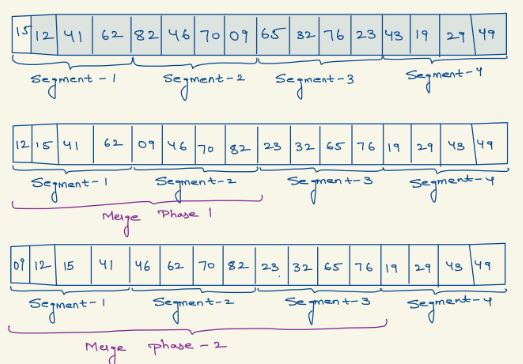
\includegraphics[width=\textwidth]{IMG1.JPG}
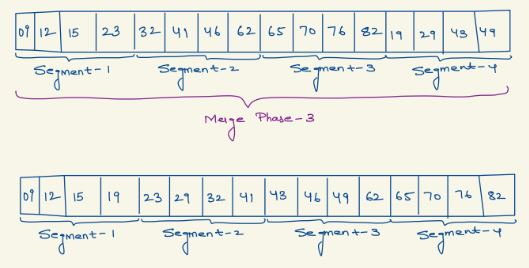
\includegraphics[width=\textwidth]{img2.JPG}
\\\\ 

\noindent\textbf{\underline {Method 2 :}}In this method once all the threads have performed the sorting then half of the total number of threads will perform the merging of the segments while the remaining half exit. This merging occurs in phases while half total number of threads exit at the end of each phase. These steps will be repeated till the array is completely sorted. 

To precisely identify the merging thread among two threads, we choose the thread with smaller id to perform the merge step while the other thread will terminate. Consider the following example: In first phase for merging of segment 1 and 2 thread 1 will perform the merging operation while thread 3 will perform the merging of segments 3 and 4. Again thread 1 will perform merging of segment 1,2 and 3,4. This is illustrated using the figures below. \\ 


%leads to the no. of sorted segments to half and half of the threads can die. Similarly quarter of the threads again perform the merging operation on the sorted segments and rest of the threads can die. 

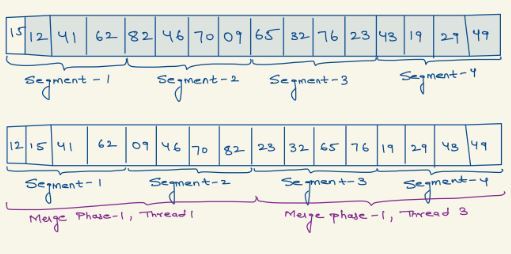
\includegraphics[width=\textwidth]{M-2,IMg1.JPG}
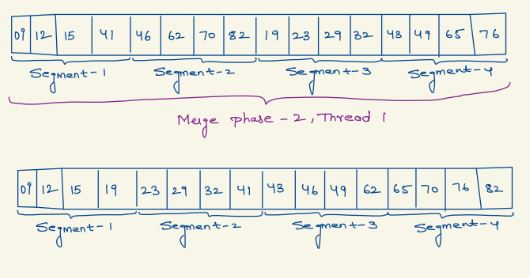
\includegraphics[width=\textwidth]{M-2,img2.JPG}\\
\noindent\textbf{\underline {Input: }}The input to the program will be a file (named inp.txt) where the first digit will be n where size of the array is $2^n$. Second digit in the file will be parameter p where the no. of segments are $2^p$
\\

\noindent\textbf{\underline {Example:}} inp.txt\\\\
5 2     \hspace{5 mm}          \textbackslash \textbackslash Size of Array $2^5$, No.of threads $2^2$\\

\noindent\textbf{\underline {Output:}} Output.txt should contain the initial array before sorting and Array after sorting in the next line. Time taken in microseconds for sorting in third line.\\


\noindent\textbf{\underline {Example:}} output.txt\\\\
8 15 22 13 16 27  \hspace{5 mm}          \textbackslash \textbackslash Array Before sorting\\
8 13 15 16 22 27  \hspace{5 mm}          \textbackslash \textbackslash Array After sorting\\
Time taken: 563 Microseconds.\\


\noindent\textbf{\underline {Report: }} As a part of this assignment, you have to prepare a report which will describe the low-level design of your program and give an analysis of its output. As a part of the report, you have to measure the performance of the algorithms by following the mentioned steps. Calculate the time taken by method 1 and 2. Don't include the timing of reading and writing to file in this. Create a graph showing the time taken by these solutions for different values of the number of threads and fixing the size of the array to $2^8$. The x-axis should be the parameter p of inp.txt i.e.2,3,4,5,6. The y-axis will include time taken by the program to terminate (in micro/milliseconds). 

Next, create another graph showing the times using both the methods while fixing the number of threads to 4. The x-axis should be the parameter n of the inp.txt i.e. 3,4,5,6,7,8. Report should include the detailed analysis of the graph.  \\\\\

\noindent\textbf{\underline {Deliverables: }}
\begin{enumerate}
    \item Report describing the low-level design of your program and analysis of output and graph. This file should be named as Asgn1$\_<$Roll No.$>$ Report.pdf
    \item Prepare a README file that contains the instructions on how to execute your submitted file. The file should be named as README.txt
    \item Name the source code file in the following format: Asgn1\_Meth1$\_<$Roll No.$>$.c and Asgn1\_Meth2$\_<$Roll No.$>$.c
    \item Upload the source code, report and README as a zip archive file and name it as Asgn1$\_<$Roll No.$>$.zip
    
\end{enumerate}
Please see the instructions given above before uploading your file. Your assignment will NOT be evaluated if there is any deviation from the instructions posted there.\\
\\
The policy for grading this assignment will be -\\
\begin{itemize}
    \item Design as described in report and analysis of the obtained results: 50\%
    \item Execution: 40\%
    \item Code documentation and indentation: 10\%.
\end{itemize}
As mentioned before, all assignments for this course has the late submission policy of a penalty of 10\% each day after the deadline.\\\\
\textbf{Kindly remember that all submissions are subjected to plagiarism checks.}

\end{document}
